\section{Introduction}

\begin{figure}[t]
    \begin{minipage}{0.48\textwidth}
        \centering
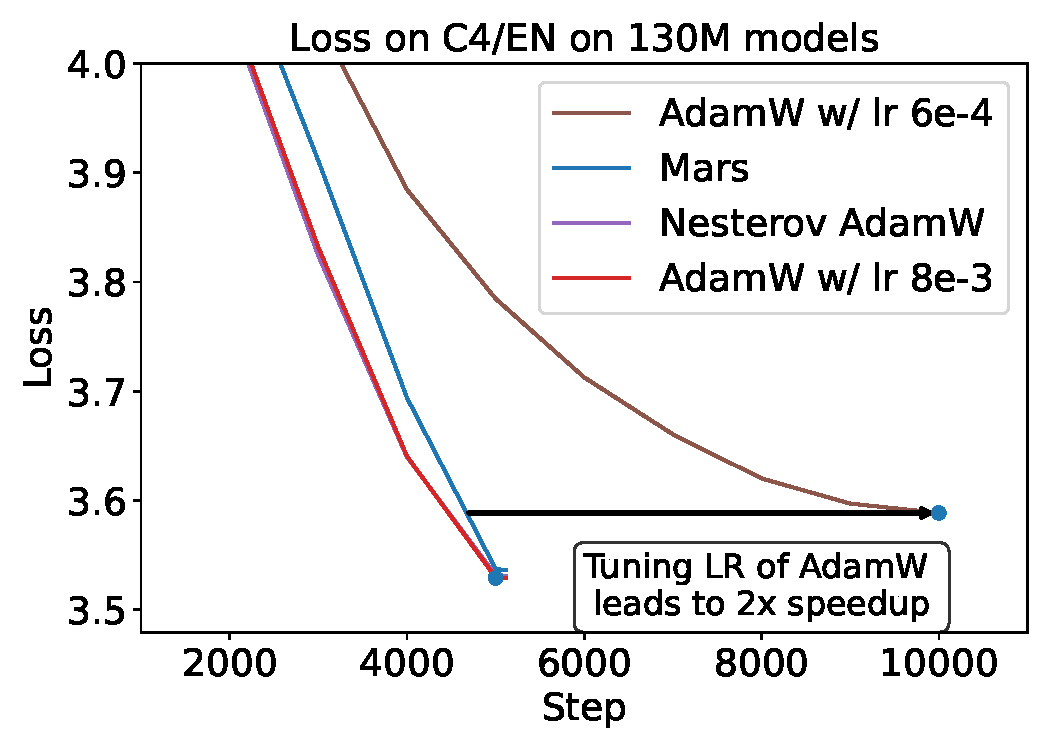
\includegraphics[width=\linewidth]{figures/fig1.pdf}
    \end{minipage}    
    \begin{minipage}{0.46\textwidth}
        \centering 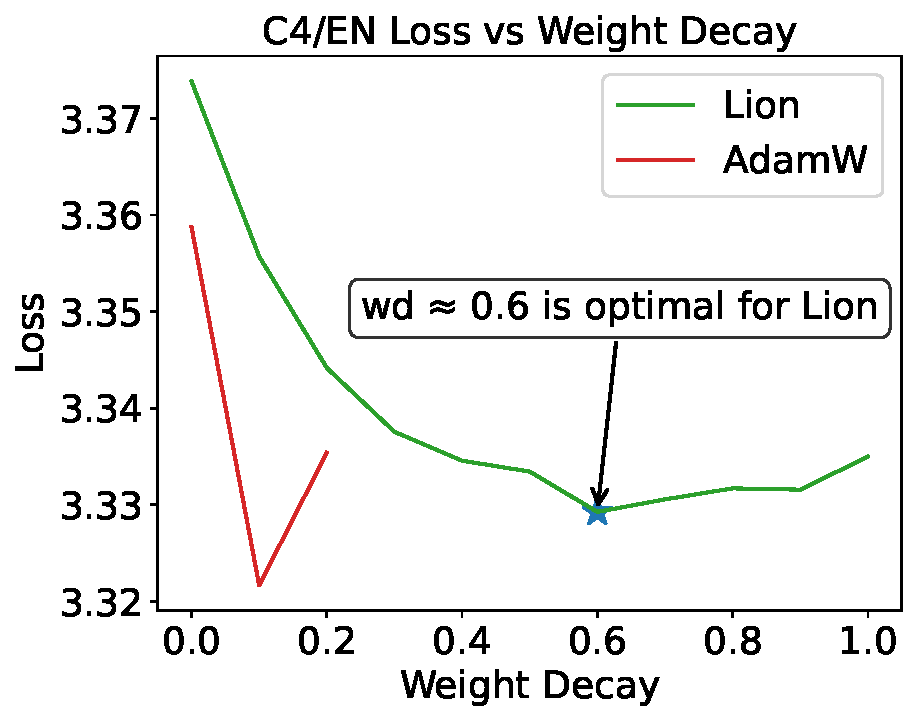
\includegraphics[width=\linewidth]{figures/wd_matters.pdf}
    \end{minipage}
    \vfill
    \begin{minipage}
        {0.46\textwidth}
            \centering
    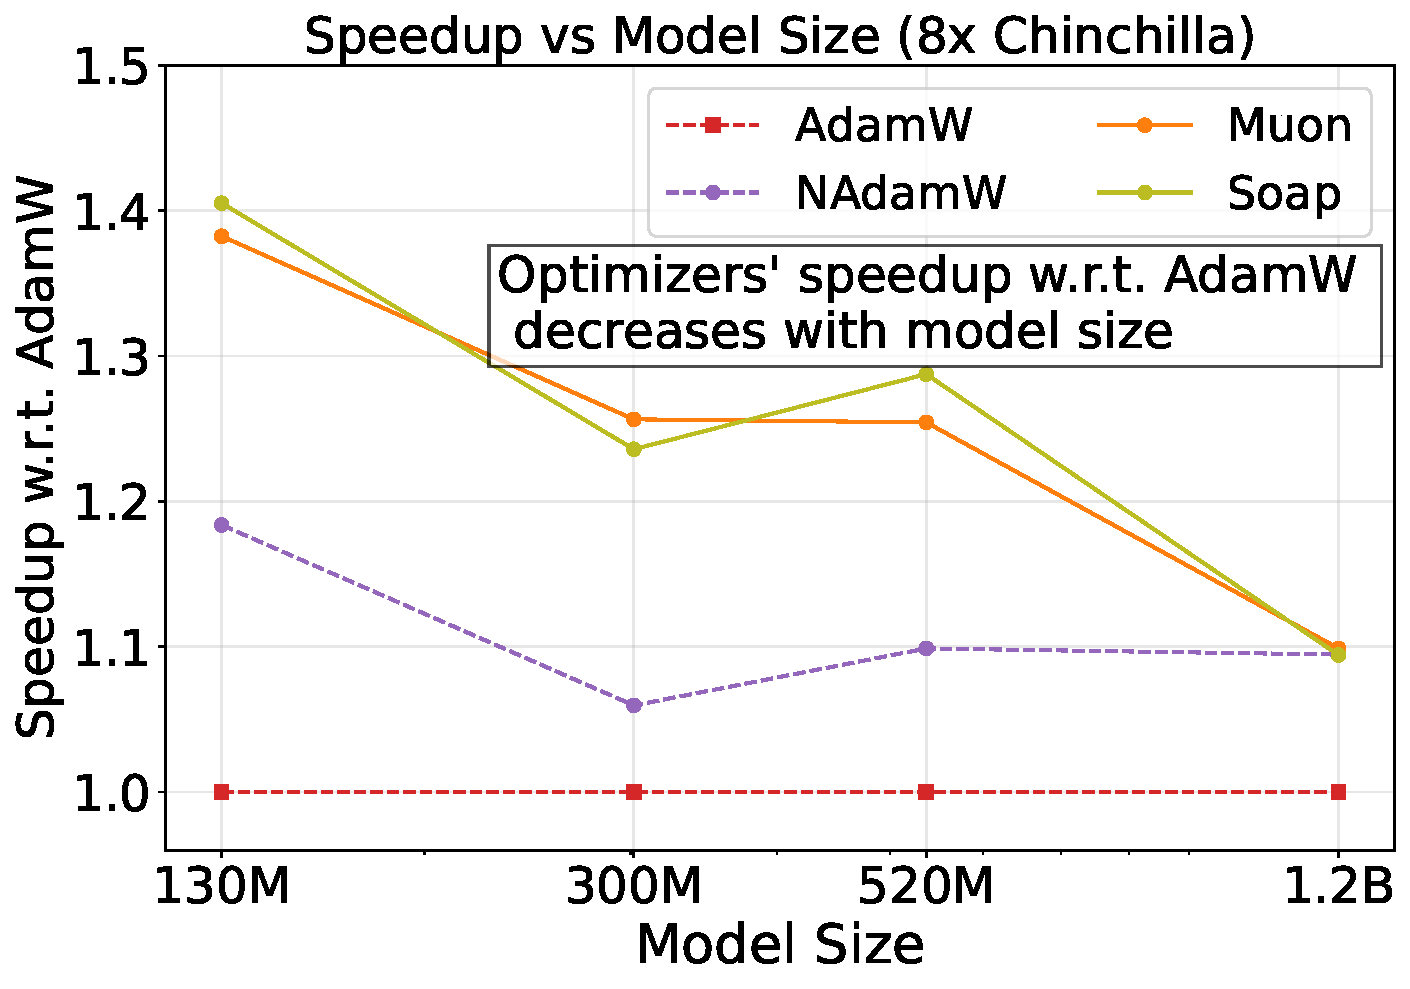
\includegraphics[width=\linewidth]{figures/speedup_vs_model_size.pdf}
        \end{minipage}
    \begin{minipage}
    {0.48\textwidth}
        \centering
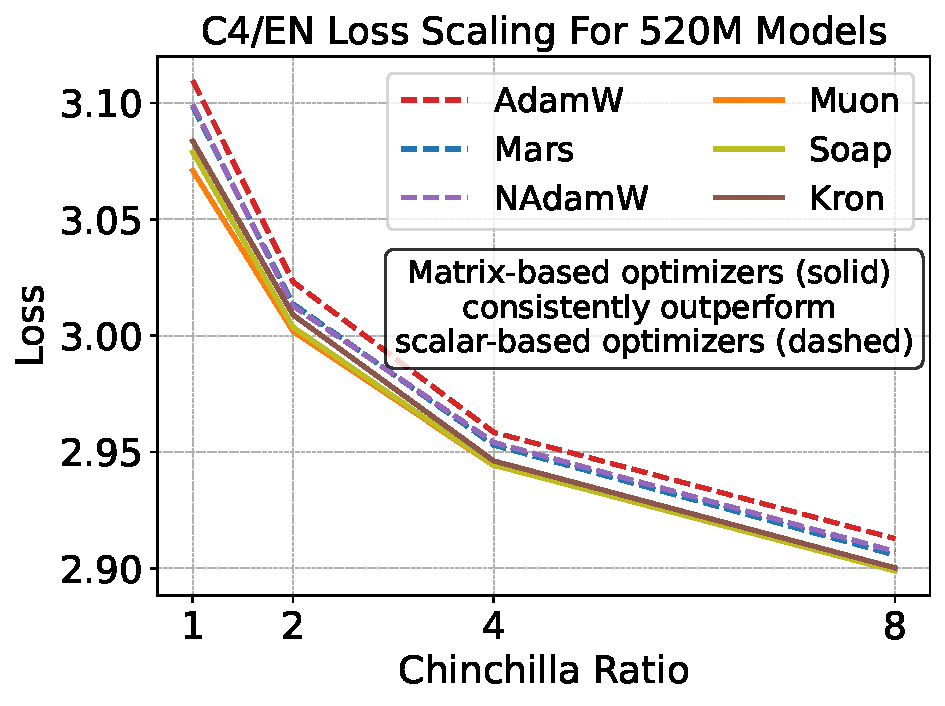
\includegraphics[width=\linewidth]{figures/optimizer_loss_scaling_520m_downsampled.pdf}
    \end{minipage}
    \caption{
    \textbf{Top Left}: {
    The commonly used AdamW baseline for optimizer design is under-tuned.} Up to a 2$\times$ speedup is achievable by tuning a single hyperparameter (learning rate) in the GPT-3 recipe~\cite{brown2020languagemodelsfewshotlearners} for a 100M model (adopted in~\cite{liu2024sophiascalablestochasticsecondorder,wen2024understandingwarmupstabledecaylearningrates,yuan2025mars,liang2025cautious,wang2025sharpnessdisparityprincipletransformers}), highlighting the importance of proper hyperparameter optimization. 
    \textbf{Top Right}: {Fixing hyperparameters across optimizers does not guarantee fair comparison.} Shared hyperparameters such as learning rate and weight decay are commonly set to a constant in previous studies. However, even conceptually similar optimizers may correspond to very different optimal hyperparameters. 
    \textbf{Bottom Left}: {Speedup decays with model size.} While some optimizers show high (1.3-1.4$\times$) speedup over AdamW on models under 1B parameters, the speedup decays with model size to only 1.1$\times$ for 1.2B parameters.  
    \textbf{Bottom Right}: {Matrix-based optimizers consistently outperform scalar-based optimizers.}
    The loss curves for three scalar-based optimizers (AdamW, Nesterov AdamW, Mars) and three matrix-based optimizers (Kron, Soap, Muon) trained with different Chinchilla ratios of data are shown. Matrix-based optimizers achieve a consistent speedup over scalar-based optimizers. Furthermore, the three matrix-based optimizers converge to a similar loss in an overtrained setting.}
    \label{fig:motivation}

    \vspace{-0.2in}
\end{figure}

Pretraining has been the most computationally expensive component in the training pipeline for large language models, accounting for over 95\% of the cost in DeepSeek V3~\cite{deepseekai2025deepseekv3technicalreport}, and the additional RL training cost in DeepSeek R1~\cite{deepseekai2025deepseekr1incentivizingreasoningcapability} is also comparatively much smaller.
Until recently, AdamW has been the standard optimizer. Recent studies have introduced novel optimizers that claim to accelerate pretraining by 1.4$\times$ to 2$\times$ compared to AdamW~\cite{liu2024sophiascalablestochasticsecondorder,vyas2025soapimprovingstabilizingshampoo,liu2025muonscalablellmtraining,yuan2025mars,liang2025cautious,wang2025sharpnessdisparityprincipletransformers,liu2025focusorderconcentratedupdating,pethick2025trainingdeeplearningmodels,ma2025swansgdnormalizationwhitening}, yet these optimizers have not yet been widely adopted in real-world pretraining~\cite{deepseekai2024deepseekllmscalingopensource,yang2025qwen3technicalreport,grattafiori2024llama3herdmodels}, with the notable exception of Kimi K2~\cite{kimiteam2025kimik2openagentic}, which uses the Muon-clip optimizer (a variant of Muon~\cite{jordan2024muon}).


We pinpoint two problems in optimizer evaluation in the evaluation process of these optimizers that both undermine confidence in new methods and limit their practical adoption. First, some baselines suffer from improperly tuned hyperparameters. Second, many experiments are confined to smaller-scale settings, leaving unanswered questions about how these optimizers perform in broader, more realistic scenarios. 



To address these issues, we benchmark eleven optimizers, including AdamW, in a rigorously controlled setup, focusing on two key questions:
\begin{enumerate}[leftmargin=*]
  \item \textbf{How to ensure hyperparameter optimality?} Previous works typically rely on manual hyperparameter selection and keep common hyperparameters such as learning rate and weight decay fixed across optimizers (e.g. \cite{liu2025muonscalablellmtraining}). This tuning process may result in a weak baseline, as the hyperparameters chosen may favor the proposed optimizers rather than for AdamW. We validate this concern by showing that tuning just one hyperparameter in the widely adopted GPT-3 recipe (introduced in~\cite{brown2020languagemodelsfewshotlearners} and used in~\cite{liu2024sophiascalablestochasticsecondorder,wen2024understandingwarmupstabledecaylearningrates,yuan2025mars,liu2025physicsskilllearning,liu2025focusorderconcentratedupdating,liang2025cautious,wang2025sharpnessdisparityprincipletransformers}) can yield a 2$\times$ speedup for pretraining (\Cref{fig:motivation}, top left). To address, this we perform coordinate descent in the hyperparameter space on N hyperparameters for all eleven optimizers, iterating until convergence across for each of six different settings for models with up to 0.5B parameters to ensure that the hyperparameters are near-optimal for each setting.
  \item \textbf{How do speedups differ across different scaling regimes?} Large language models are trained in different regimes: depending on the model size, the data-to-model ratio (the number of tokens over the number of parameters) can range from $1$ to more than $50$ times the Chinchilla optimal (about $20$ based on~\cite{hoffmann2022trainingcomputeoptimallargelanguage}). Typical optimizer experiments in $1\times$ Chinchilla optimal regimes raise concerns about a new optimizer's effectiveness in high data-to-model ratio. To address this, we benchmark the optimizers in four distinct data-to-model ratios (1$\times$, 2$\times$, 4$\times$ and 8$\times$ the Chinchilla optimal regime) and scale up to  1.2B parameter models (following~\cite{everett2024scalingexponentsparameterizationsoptimizers,zhang2025doescriticalbatchsize}).
\end{enumerate}

Concretely, we employ the Llama 2 architecture \cite{touvron2023llama2openfoundation,grattafiori2024llama3herdmodels} 
(ranging from 0.1B to 1.2B parameters) and a data mixture similar to OLMo 2's~\cite{olmo20252olmo2furious}. We focus on the final validation loss on the C4‐EN mixture as a known proxy for downstream performance~\cite{bhagia2024establishingtaskscalinglaws}, while also tracking exact downstream performance on various benchmarks. As previous works~\cite{vyas2025soapimprovingstabilizingshampoo,liu2025muonscalablellmtraining} show that the step-wise computation overhead of matrix-based optimizers can be reduced to under $10\%$ through proper implementation, we primarily compare algorithms by the number of tokens needed to reach a given loss.

Our empirical results show the necessity of careful hyperparameter tuning and end-of-training evaluations across a range of model scales and data-to-model ratios:
\begin{enumerate}
[leftmargin=*]
  \item \textbf{Hyperparameter transfer between optimizers is non-trivial.} Even similar optimizers may need very different hyperparameters (e.g., Lion's optimal weight decay $\approx$0.6 vs.\ AdamW's $\approx$0.1, \Cref{fig:motivation}, top right), so fixing hyperparameters across optimizers can lead to unfair comparisons.
    \item \textbf{The speedup of new optimizers is lower than claimed and diminishes with model size.} Many reported speedups of 2$\times$ simply reflect a weak baseline. Against our well-tuned AdamW baseline, the speedup of alternative optimizers does not exceed 1.4$\times$(\Cref{fig:speedup}). Furthermore, while new optimizers such as Muon and Soap show 1.3$\times$ speedups for small models (0.1B), the speedups diminish to around 1.1$\times$ for 1.2B parameter models at 8$\times$ Chinchilla Ratio (\Cref{fig:motivation}, bottom left), a regime that is not tested in previous works studying the scaling law of these optimizers \footnote{The original Soap paper~\cite{vyas2025soapimprovingstabilizingshampoo} investigate model sizes up to 0.6B parameters. and Kimi's paper on Muon~\cite{liu2025muonscalablellmtraining} only considers $1\times$ Chinchilla regime.}.
    \item \textbf{Early-stage loss curves can mislead significantly.} During learning rate decay, loss curves of different optimizers may cross multiple times (\Cref{fig:necessity}), so judging optimizers using intermediate checkpoints may result in a different ranking than comparing models at the target training budget.
\end{enumerate}


Our benchmarking also reveals new insights about optimizer design: 

\begin{enumerate}[leftmargin=*]
    \item \textbf{Matrix-based optimizers consistently outperform scalar-based optimizers for small models.} 
    \emph{Scalar-based optimizers} (e.g., AdamW, Lion, Mars, etc.) update each parameter individually using scalar operations. After proper tuning, all scalar-based optimizers achieve similar optimization speeds to AdamW, with an average speedup ratio of less than 1.2$\times$. \emph{Matrix-based optimizers} (e.g., Kron, Muon, Soap, etc.) leverage the inherent matrix structure of neural network parameters and precondition gradients using matrix multiplication. Despite their diverse update rules, matrix-based optimizers all deliver approximately a 1.3$\times$ speedup over AdamW (\Cref{fig:motivation}, bottom right) for models under 520M parameters.
    
    
    \item \textbf{Optimal choice of optimizer shifts depends on data-to-model ratios.} A winner in the $1\times$ Chinchilla regime may be suboptimal when data-to-model ratio increases. For example, while Muon is consistently the best optimizer in smaller Chinchilla ratio regimes, it is outperformed by Kron and Soap when the data-to-model ratio increases to 8x or larger (\Cref{fig:speedup,fig:case}). 
\end{enumerate}

